%##############################################%
% aspectosgerais < Desenvolvimento             %
% consideracoes < Metodologia                  %
% textoepostexto < Resultados                  %
% elementosdotexto < Conclusão                 %
%##############################################%


%Descrever primeiro o problema de segurança (MiddleMan e outros tipos de ataques)
%Introduzir o conceito de criptografia e comunicação segura
%Falar sobre autoridades certificadoras, centros de distribuição de chaves
%Certificados digitais e o X.509

\chapter[Fundamentação Teórica]{Fundamentação Teórica}

	Neste capítulo a principal meta é inteirar o leitor sobre a importância do uso e da qualidade de certificados digitais, de forma correta. Inicialmente serão apresentados detalhes sobre o que é comunicação segura, e a criptografia. Em seguida, serão abordados e apresentados os detalhes da criptografia, tanto simétrica quanto assimétrica. Por fim, serão discutidos certificados digitais e sua importância, assim como seu uso.

\section[Criptografia e Protocolos]{Criptografia e Protocolos}
	No contexto da computação, as redes de computadores têm se tornado cada vez maiores, esperasse um trânsito elevado de informações, e o uso dessas redes de computadores para a troca de informações é esperado. 
	
	Nesse quadro, dois indivíduos pretendem trocar informações e desejam trocar suas mensagens de forma segura, eles desejam confidencialidade. Para esse fim, eles podem escolher utilizar a criptografia. A criptografia em si, possui muitos fins:

	\begin{itemize}
		\item \textbf{Confidencialidade} - Ocultar a informação contida em uma mensagem, de forma que apenas o emissor e o receptor conheçam seu conteúdo.
		\item \textbf{Autenticação} - Dar a possibilidade do recebedor identificar a origem de uma mensagem.
		\item \textbf{Integridade} - Permitir que o recebedor tenha certeza que aquela mensagem não foi modificada por um terceiro.
		\item \textbf{Não-Repudiação} - Um remetente não deve ser capaz de negar falsamente o envio de uma mensagem.
	\end{itemize}

	Os indivíduos de nosso exemplo serão, figurativamente, chamados de \textit{A} e \textit{B}, e suas mensagens serão chamadas de \textit{mA} e \textit{mB}, respectivamente. Chamando a mensagem original, \textit{mA}, de \textbf{texto plano}, ela pode ser alterada através de \textit{encriptação} para gerar um \textbf{texto cifrado}, \textit{enA}, e retornará ao seu estado original passando por uma \textit{desencriptação} \cite[p.~15]{schneier96}.

	\begin{figure}[h]
		\centering
		\label{img01}
		\caption{Processo de Encriptação e Decriptação}
		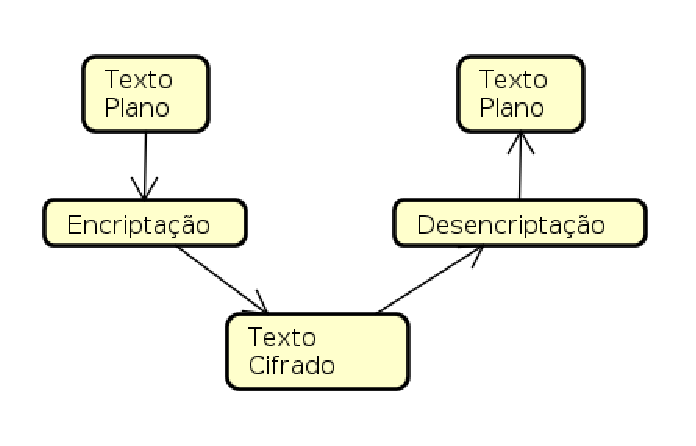
\includegraphics[keepaspectratio=true,scale=0.5]{figuras/proc.eps}
	\end{figure}

	Um algoritmo de criptografia pode ser chamado de cipher code. Existem cipher codes cuja segurança depende de seu segredo, e existem outros cuja segurança depende do segredo de valores denominados chaves.
	
	Porém, a comunicação em si pode não estar completamente segura apenas com o uso da criptografia, caso um algoritmo ou chave de encriptação secretos sejam expostos, esses casos caracterizam quebras de segurança \cite[p.~399]{stallings11}:
	
	\begin{itemize}
		\item \textbf{Quebra Total} - Um indivíduo externo descobriu a \textit{chave} do algoritmo.
		\item \textbf{Dedução Global} - Um indivíduo externo encontra um algoritmo equivalente, sem conhecer a \textit{chave}.
		\item \textbf{Dedução Seletiva} - Um indivíduo externo consegue acesso ao \textit{texto plano} de um \textit{texto cifrado}.
		\item \textbf{Dedução Existencial} - Um indivíduo externo tem acesso a uma parcela de informação da \textit{chave} ou do \textit{texto plano}. 
	\end{itemize}

	Para reduzir as chances de possíveis vazamentos de mensagens, é possível seguir protocolos de comunicação, esses \textit{protocolos} se fazem úteis tanto para padronizar a forma como as informações são trocadas quanto para ajudar na interpretação do que está sendo falado pelos envolvidos.
	
	A criptografia em si pode ser reforçada por outros métodos que tornariam a troca de mensagens ainda mais segura, é possível então que os indivíduos insiram na sua forma de comunicação um \textbf{protocolo}. Um \textit{protocolo} é um processo realizado pelos participantes de uma atividade (no caso a comunicação) para realizar essa atividade, sendo que esse processo apresenta passos bem definidos e que devem ser seguidos \cite{schneier96}.
	
	Um \textbf{protocolo criptográfico} é aquele que envolve protocolo que envolve criptografia \cite[p.~31]{schneier96}, como por exemplo o protocolo de comunicação \textit{HTTPS}. Os protocolos ajudam a gerar confiança entre os envolvidos, eles podem exigir uma troca de chaves secretas ou uma linguagem específica. Isso pode ser feito para convencer os envolvidos de que são quem verdadeiramente afirmam. Deve-se ter em mente, também, que o protocolo deve se limitar ao que se propõe em cada caso, para aumentar a segurança dos indivíduos.
	
	Como exemplo é possível imaginar dois estranhos se vendo pela primeira vez, imagine que o protocolo social que se segue é cumprimentar as pessoas com um aperto de mão. Caso os dois estranhos se encontrem na rua, e se cumprimentem com um aperto de mãos, eles dirão um ao outro seus respectivos nomes, e iniciarão uma conversa. Caso o aperto de mãos não ocorra, isso seria uma quebra de protocolo, e a comunicação entre eles terminaria ali.

\section[Algoritmos e Chaves]{Algoritmos e Chaves}

	Existem duas formas mais populares de se tratar com chaves de segurança, mantendo-as em segredo (\textit{chaves secretas ou privadas}), na \textbf{criptografia de chave simétrica}, ou tornando-as acessíveis (\textit{chaves públicas}) em par com chaves privadas, na \textbf{criptografia de chave assimétrica}. Cada um dos casos apresenta suas próprias vantagens, e desvantagens, sendo possível trabalhar com ambos objetivando uma troca segura de informações.
	
	Nos algoritmos de chave privada, a chave é compartilhada pelos envolvidos na troca de informações. Utilizando de um mesmo algoritmo conhecido, eles irão enviar suas mensagens, e recebê-las, utilizando uma mesma chave secreta para o processo de encriptar e \textit{desencriptar} as informações trocadas. Na atualidade, é comum que essas chaves privadas sejam monitoradas por \textbf{KDCs} (\textit{Key Distribution Centers}), \textbf{Centros de Distribuição de Chaves}, afim de arbitrar a distribuição e consenso em relação à chave utilizada em uma troca.

	\begin{figure}[h]
		\centering
		\label{img02}
		\caption{Processo de Encriptação e Desencriptação com Chave Privada}
		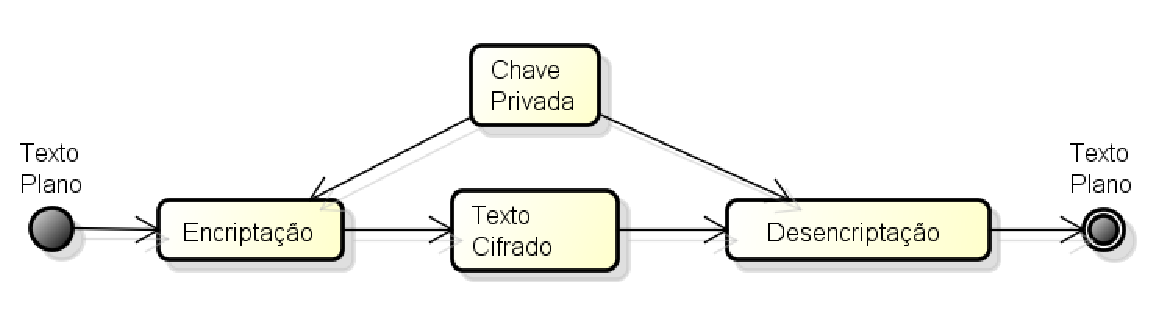
\includegraphics[keepaspectratio=true,scale=0.5]{figuras/img01.eps}
	\end{figure}

	Já os algoritmos de chave pública seguem uma ideia diferente, existe uma chave conhecida publicamente e uma chave secreta, idealmente conhecida apenas pelo usuário. Através da encriptação utilizando a chave pública de um indivíduo, os algoritmos de chave assimétrica irão garantir que apenas a chave privada do indivíduo seja capaz de desencriptar a mensagem. Da mesma forma, utilizar a própria chave privada para encriptar um conteúdo irá garantir que apenas a chave pública seja utilizada para desencriptar corretamente aquela mensagem, atestando a origem daquela mensagem.

	\begin{figure}[h]
		\centering
		\label{img03}
		\caption{Processo de Encriptação em Chave Pública}
		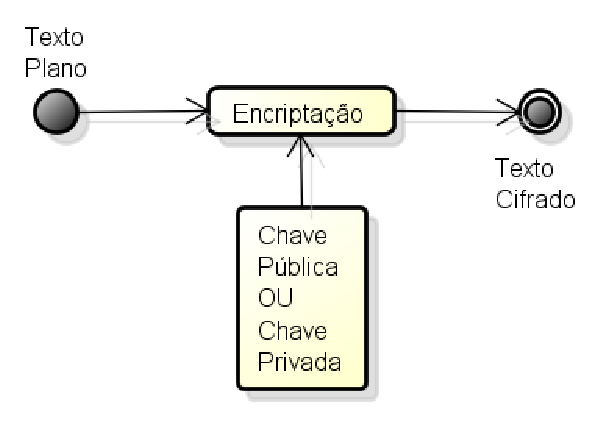
\includegraphics[keepaspectratio=true,scale=0.5]{figuras/encript.eps}
	\end{figure}
	
	\begin{figure}[h]
		\centering
		\label{img04}
		\caption{Processo de Desencriptação em Chave Pública}
		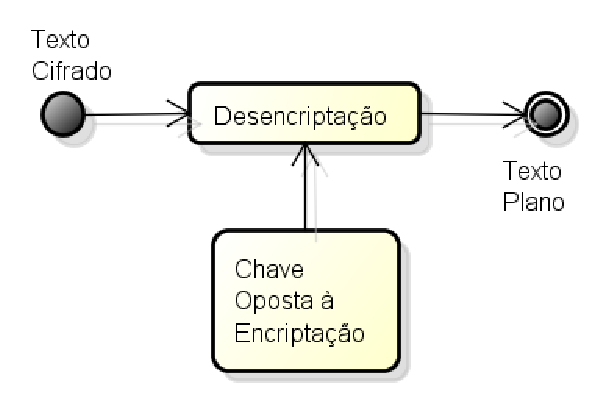
\includegraphics[keepaspectratio=true,scale=0.5]{figuras/desencript.eps}
	\end{figure}

	Nesse contexto, a encriptação com a própria chave privada serviria como meio de assinar um conteúdo, de forma a garantir a autenticidade e a não-repudiação. Em se tratando de uma comunicação verdadeiramente séria, é possível empregar mais de uma encriptação, com o objetivo de garantir que um conteúdo seja lido apenas pelo destinatário, e que seja provada a identidade do remetente.
	
	Entretanto, para garantir  que essas trocas sejam feitas, e que haja consenso em como encriptar e desencriptar essas informações, é necessário que os algoritmos utilizados no processo sejam conhecidos por ambas as partes. Diferente de algoritmos que se tornam seguros através do segredo do algoritmo em si, algoritmos que utilizam chaves, geralmente, tem sua segurança embasada nas chaves em si, sendo os algoritmos públicos. Historicamente, existem diversos algoritmos de criptografia conhecidos e utilizados, vale citar dois desses algoritmos: o DES e o RSA.
	
	Um dos primeiros algoritmos utilizados em larga escala, o DES (Data Encryption Standard) na verdade se trata de um padrão, detentor do algoritmo DEA (Data Encryption Algorithm). Em seu funcionamento, esse algoritmo adota a Função de Feistel, que realiza a encriptação através de quatro estágios. A função-F (como é conhecida a função de Feistel) é repetida diversas vezes dentro do algoritmo, de forma que ao final de diversas repetições será alcançado o texto cifrado.
	
	\begin{figure}[h]
		\centering
		\label{img05}
		\caption{Processo de Encriptação do DEA \cite{DEA}}
		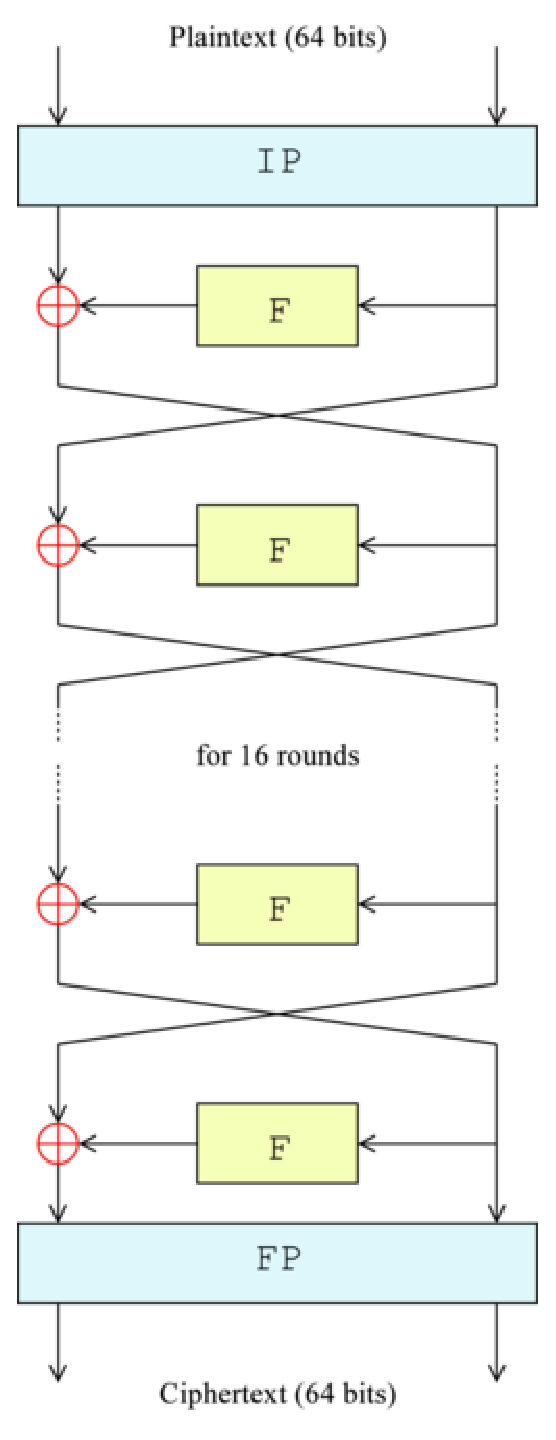
\includegraphics[keepaspectratio=true,scale=0.3]{figuras/DES.eps}
	\end{figure}
	
	Já o RSA, nomeado assim em referência aos seus criadores, é utilizado para a encriptação utilizando chaves assimétricas. Seu funcionamento difere, pois certas formalidades são exigidas para gerar as chaves a serem utilizadas nesse algoritmo. As chaves utilizadas dependem de dois números primos grandes (o que matematicamente diminui as chances de uma quebra de segurança) que irão ser utilizados em sua geração, que se dá de forma que:
	
	\begin{enumerate}
		\item Dois números primos grandes \textbf{p} e \textbf{q}, são escolhidos;
		\item É calculado $\textbf{n} = pq$;
		\item Utiliza-se a função-$\varphi$ onde $n: \varphi(n) = (p-1)(q-1)$;
		\item É escolhido um valor \textbf{e} (inteiro) maior que 1 e menor que $\varphi(n)$, de forma que \textit{e} e $\varphi(n)$ sejam primos entre si.
		\item Calcula-se \textbf{d} como inverso multiplicativo de \textit{e}, onde mod($\varphi(n)$)
	\end{enumerate}
	
	Assim gerando uma chave pública através do par \textit{(e, n)}, e uma chave privada do conjunto \textit{(p, q, d)} ou apenas \textit{(d)}, o segundo caso sendo uma abordagem mais lenta, pois o desencriptador não conhece os primos originais. A encriptação e desencriptação se dão, respectivamente, pelas fórmulas: \textit{(onde m é o texto plano, e c é o texto cifrado)}
	
	\begin{enumerate}
		\item $c = m^e mod n$
		\item $m = c^d mod n$
	\end{enumerate}
	
	Existem muitos algoritmos de cifração de chave pública, porém a maioria é impraticável por questões de desempenho. É importante notar que a complexidade envolvida nesses algoritmos desse tipo se deve a existência da própria chave pública, pois os procedimentos envolvidos para gerá-la não são simples, nem mais eficientes que algoritmos simétricos \cite{stallings11}. Para se trabalhar com esse tipo de sistema, é necessário que o algoritmo e a chave pública não sejam suficientes para descobrir a chave privada \cite{pkcs8}. Essa mesma capacidade de gerar chaves públicas em par com chaves privadas permite que algoritmos assimétricos gerem um texto cifrado a partir de um texto plano usando uma chave pública, e que a chave privada seja a única capaz de decifrar aquele texto cifrado gerado \cite{pkcs1}.
	
	Originalmente o que foi proposto por Diffie-Hellman para as aplicações de algoritmos de chave pública permitia apenas a Troca de Chaves, já na abordagem RSA se tornou possível utilizar Assinaturas Digitais \cite[p.~12]{pkcs1} e esquemas de Encriptação/Decriptação \cite[p.~15]{pkcs1}; o uso do RSA se tornou difundido pela sua aplicabilidade e a impraticabilidade de ataques por conta do tamanho e administração de suas chaves.
	
	Pela capacidade de gerar novas chaves públicas, e possuir uma chave privada, os algoritmos assimétricos servem aos seguintes propósitos \cite[p.~275]{stallings11}:
	
	\begin{itemize}
		\item \textbf{Encriptação/Decriptação} - O remetente pode encriptar uma mensagem com a \textit{chave pública} do receptor.
		\item \textbf{Assinatura Digital} - Um remetente pode assinar uma mensagem com sua \textit{chave privada}. A assinatura pode ser alcançada por métodos diferentes, de acordo com os \textit{protocolos} utilizados.
		\item \textbf{Troca de Chaves} - Duas entidades em conjunto geram uma \textbf{chave de sessão}. Assim como na assinatura digital, existem diversas aproximações para que isso seja alcançado. 
	\end{itemize}

\section[Certificados Digitais]{Certificados Digitais}

	No contexto da comunicação segura, a ideia de saber a identidade do outro indivíduo é essencial; Não é desejável que um desconhecido se faça passar pela receptor, ou mesmo pelo emissor, um \"homem do meio\". Para garantir essa comunicação de um para um, é desejável que sejam apresentadas credenciais que garantam que a mensagem foi transmitida sem desvios, e pelo emissor esperado. Acerca disso, Schneier exemplifica:

	\textit{\lq\lq Um certificado público é a chave pública de alguém, assinada por alguém confiável. Certificados são usados para frustar tentativas de substituir uma chave por outra [879]. O certificado de Bob, numa base de dados de chaves-públicas, possui muito mais que sua chave pública. Ela contém informações sobre Bob -seu nome, endereço, e por aí vai- e é assinado por alguém em quem Alice confia: Trent (comumente conhecido como uma autoridade certificadora, ou AC)}...\rq\rq\ \cite[p.~163, com adaptações]{schneier96}.

	Em suma, o que o autor diz é que a forma mais simples de atestar a identidade de uma pessoa é utilizando um \textbf{certificado de chave pública}. Pensando numa situação onde aparecem os indivíduos \textbf{A}, \textbf{B}, e \textbf{C}, um certificado apresenta várias informações sobre um \textit{indivíduo A}, e é assinado por um \textit{indivíduo C} externo, para que o \textit{indivíduo B} passe a confiar no \textit{indivíduo A}. Para que esse certificado seja confiável e válido, é necessário que o \textit{indivíduo A} e o \textit{indivíduo B} confiem no \textit{indivíduo C}. No caso o indivíduo C seria então conhecido como uma \textbf{Autoridade Certificadora}.

	Para que esses certificados possam seguir um padrão, foram criados os \textbf{Public-Key Cryptography Standards}, ou \textit{PKCS}, e dentre elas, especificamente a \textit{PKCS \#10} \cite{pkcs10}, cujo objetivo é padronizar os dados contidos em \textit{certificados digitais}, assim como definir quais tipos de informações devem estar contidas em um \textit{certificado digital} e o modelo que deve ser seguido para se requisitar um. O certificado funciona da seguinte forma \ref{img05}:

	\begin{figure}[h]
		\centering
		\label{img06}
		\caption{Certificado de Chave Pública em Uso \cite[p.~430]{stallings11}}
		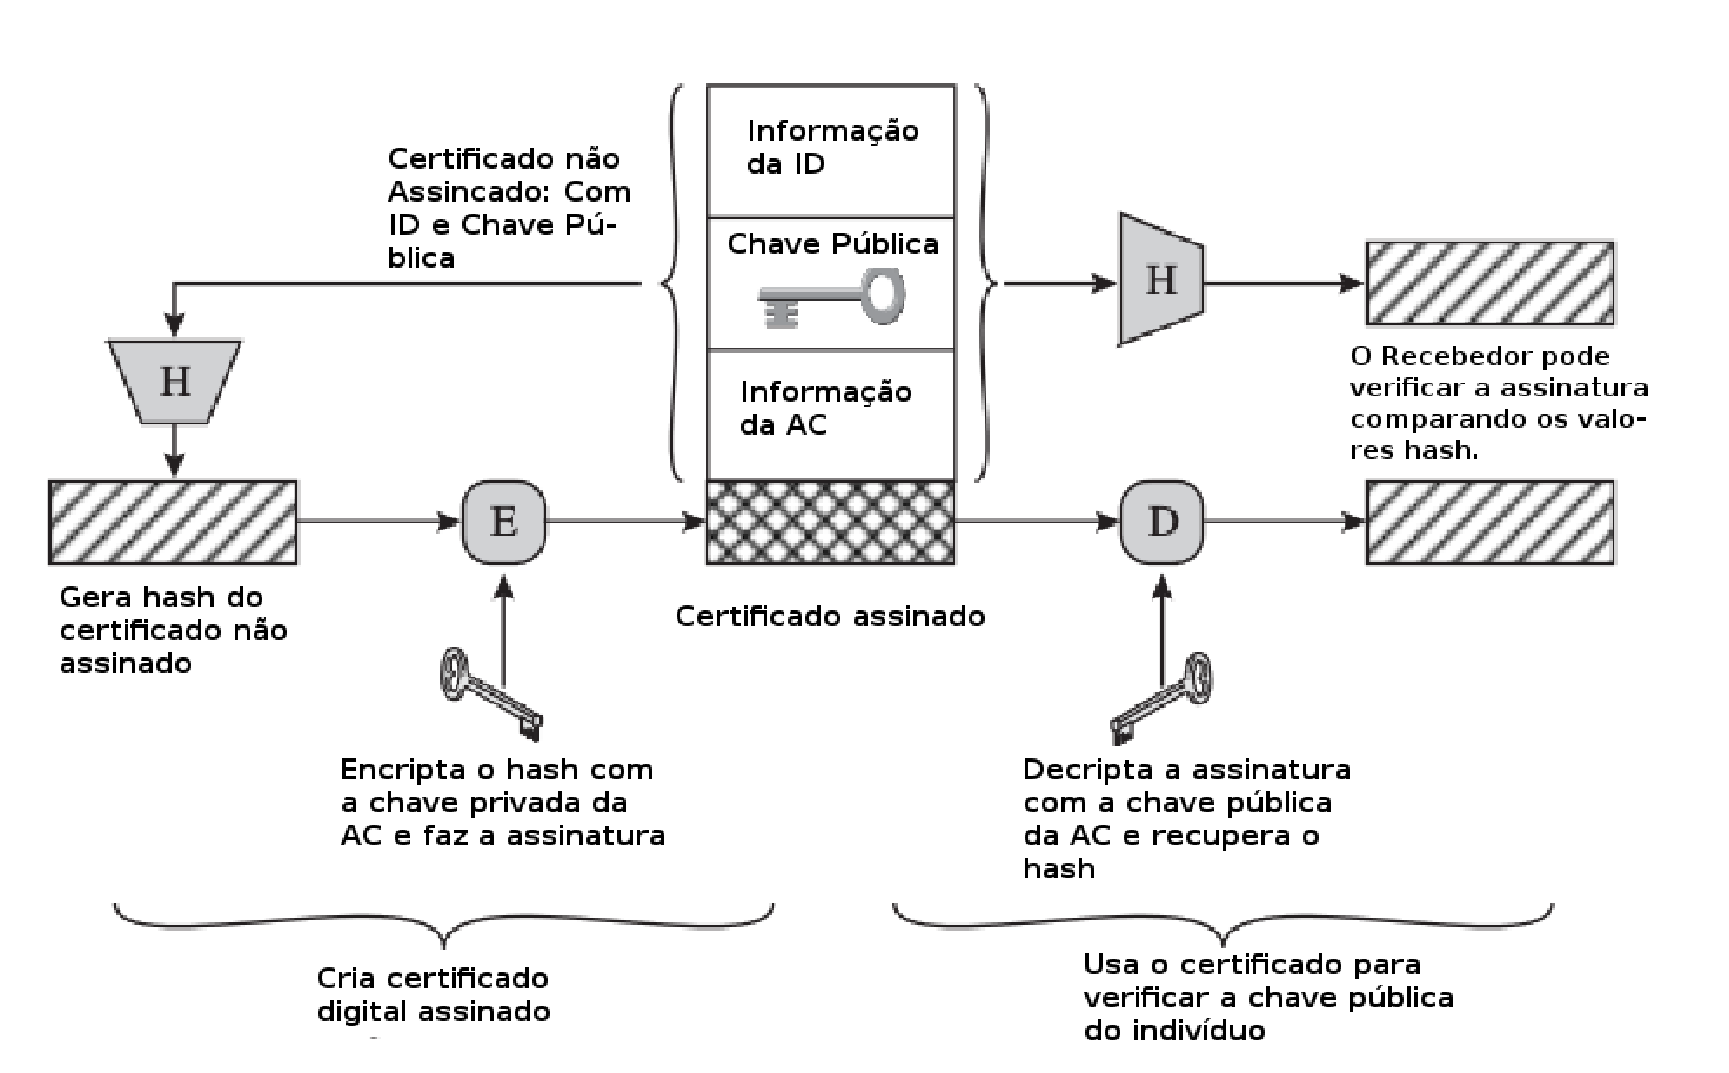
\includegraphics[keepaspectratio=true,scale=0.46]{figuras/img05.eps}
	\end{figure}
 
	Esses certificados utilizam o padrão \textbf{X.509}. O \textit{X.509} não dita um \textit{cipher} específico, entretanto ele aconselha que seja utilizado o \textit{RSA} para a implementação da \textit{criptografia de chave pública} e das \textit{assinaturas digitais}. Na figura abaixo se observa a estrutura de um certificado:

	\begin{figure}[h]
		\centering
		\label{img07}
		\caption{Certificado X.509 \cite[p.~431]{stallings11}}
		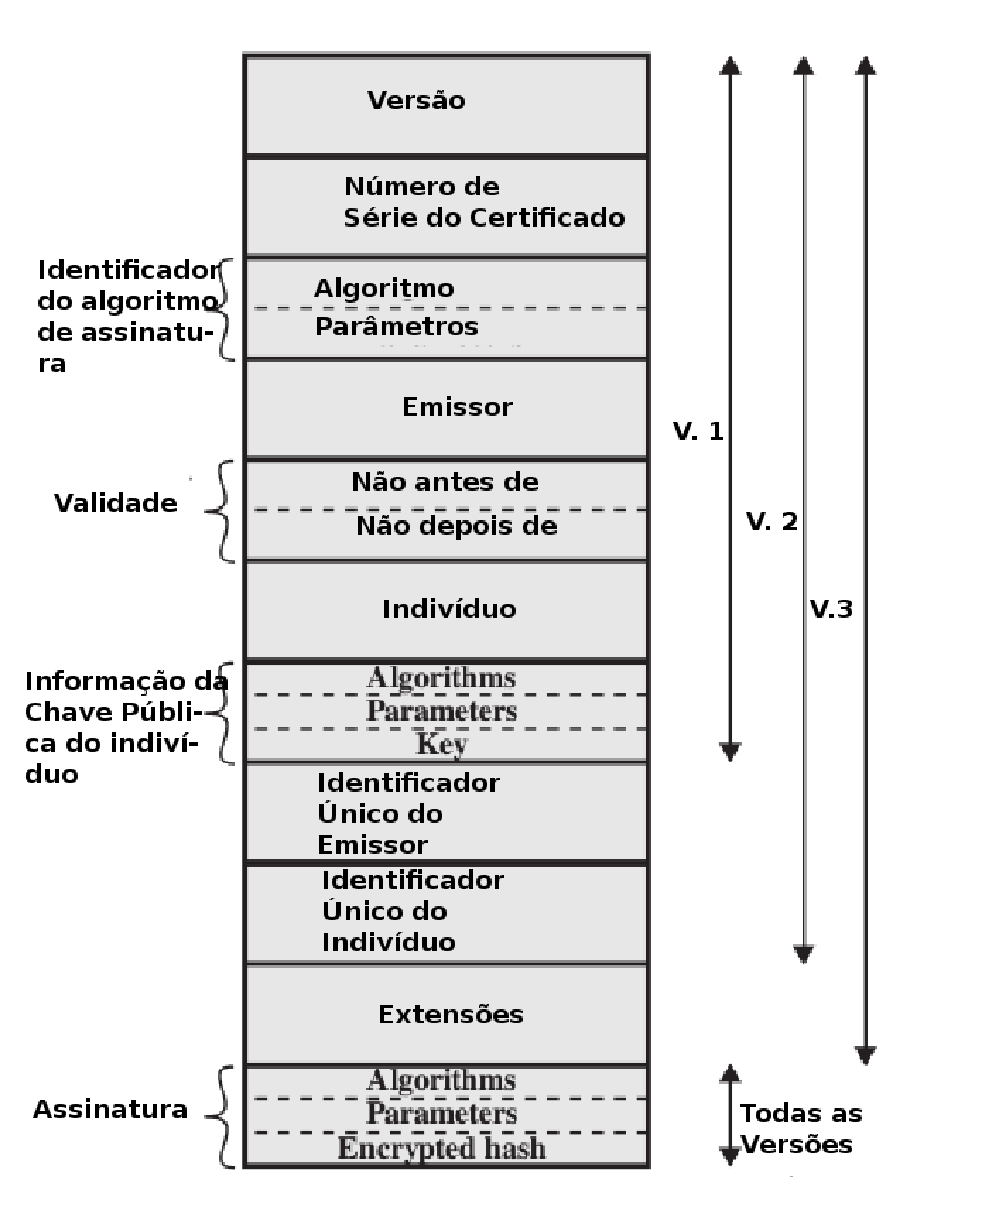
\includegraphics[keepaspectratio=true,scale=0.7]{figuras/img04.eps}
	\end{figure}

	E esses certificados \textit{X.509} podem ainda se mostrar de duas formas, em formato \textbf{DER} ou \textbf{PEM}. Quando se encontram em codificação \textit{DER} (\textit{Distinguished Encoding Rules}), esses certificados se apresentam em formato binário, legíveis apenas através dos devidos interpretadores por parte da máquina. Por outro lado, os \textit{PEM} (\textit{Privacy Enhanced Mail}) usam codificação \textbf{ASCII}, facilitando sua interpretação e leitura, assim como a distinção das informações contidas em seu corpo.

	Como já foi dito, a ideia de um certificado é atestar a identidade dos indivíduos envolvidos numa transação de informações. Para isso, pode ser necessário que uma terceira parte se envolva, caso aqueles que se comunicam não conheçam os certificados um do outro de antemão, e esse terceiro envolvido seria uma autoridade certificadora, de confiança mútua entre os envolvidos. Essa terceira entidade, geralmente, conhecida como \textbf{Autoridade Certificadora}, é responsável por emitir e assinar os certificados digitais que circulam em determinados domínios. Por exemplo, no domínio brasileiro, temos a \textbf{AC Raiz}, como autoridade certificadora raiz, definindo quem pode ser visto como um agente certificador e emitindo certificados para tais indivíduos.

	Abaixo, podemos observar a estrutura simplificada da árvore de certificação brasileira.

	\begin{figure}[h]
		\centering
		\label{img08}
		\caption{Árvore Simplificada de Autoridades Certificadoras Brasileiras \cite{itiICPBRASIL}}
		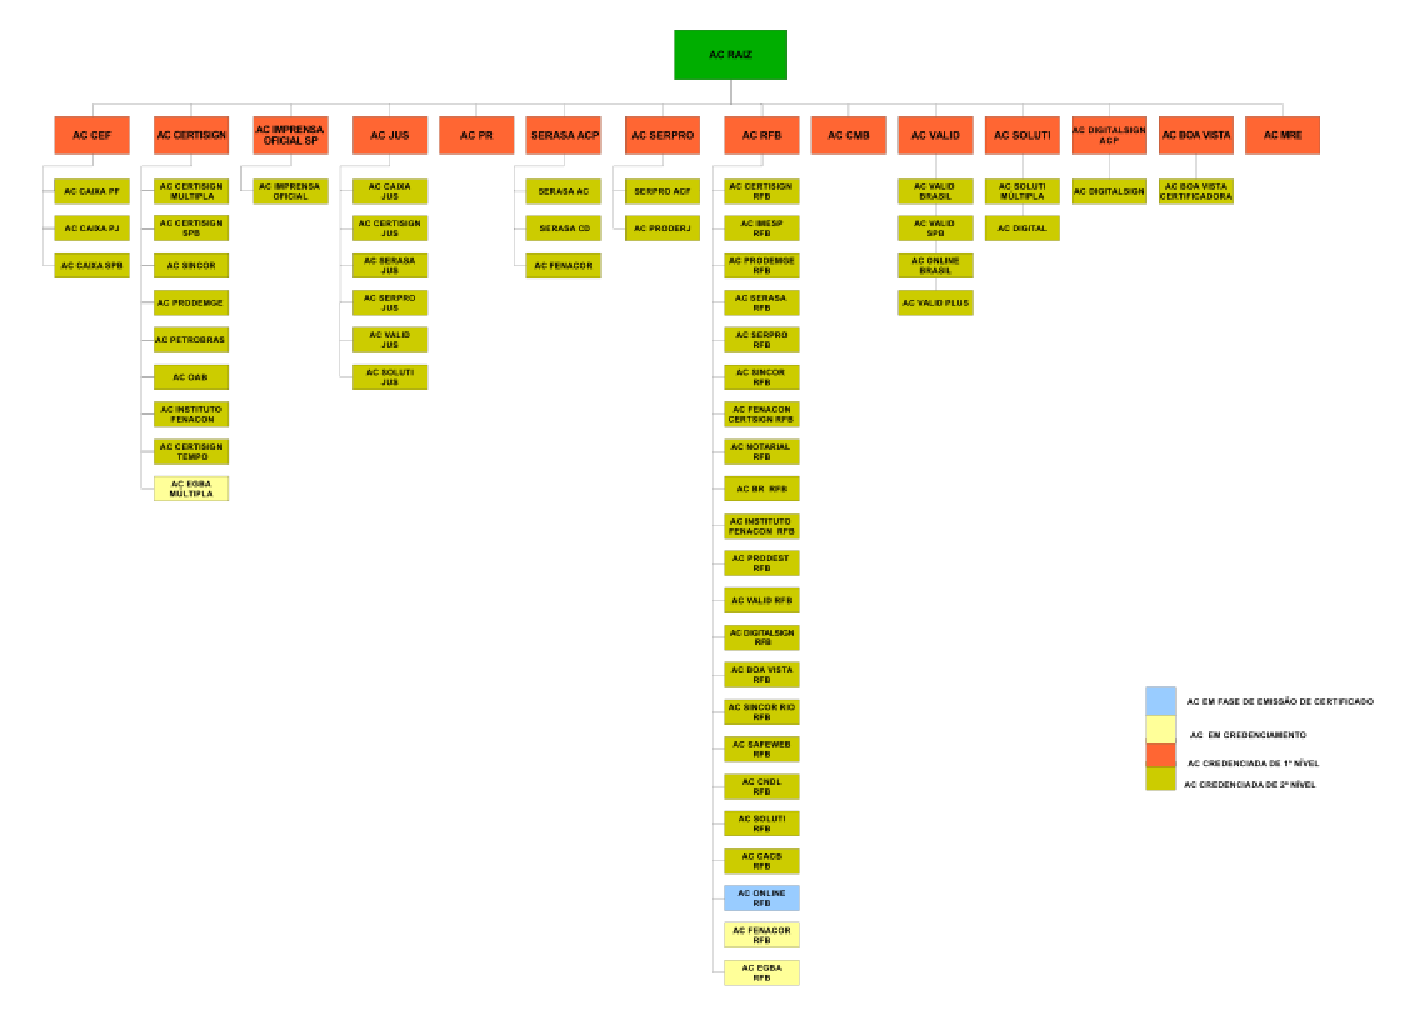
\includegraphics[keepaspectratio=true,scale=0.7]{figuras/certBR.eps}
	\end{figure}

	Entretanto, esses certificados também podem apresentar erros, ou falhas, e comprometer a confiabilidade da troca de informações por diversos fatores, que podem acarretar em quebras de segurança, esses erros são explicitados através de verificações realizadas por ferramentas de geração e análise de certificados digitais (entre outras funções). Abaixo, a tabela de erros identificáveis através da ferrammenta \textbf{OpenSSL}. 

	\begin{center}
		\begin{longtable}{c>{\em}l}
		\toprule
		\textbf{Valor Associado} & \textbf{Retorno} \\ \midrule
		0 & ok \\ 
		\rowcolor[gray]{0.9}
		2 & unable to get issuer certificate \\ 
		3 & unable to get certificate CRL \\ 
		\rowcolor[gray]{0.9}
		4 & unable to decrypt certificate's signature \\ 
		5 & unable to decrypt CRL's signature \\ 
		\rowcolor[gray]{0.9}
		6 & unable to decode issuer public key \\ 
		7 & certificate signature failure \\ 
		\rowcolor[gray]{0.9}
		8 & CRL signature failure \\ 
		9 & certificate is not yet valid \\ 
		\rowcolor[gray]{0.9}
		10 & certificate has expired \\ 
		11 & CRL is not yet valid \\ 
		\rowcolor[gray]{0.9}
		12 & CRL has expired \\ 
		13 & format error in certificate's notBefore field \\ 
		\rowcolor[gray]{0.9}
		14 & format error in certificate's notAfter field \\ 
		15 & format error in CRL's lastUpdate field \\ 
		\rowcolor[gray]{0.9}
		16 & format error in CRL's nextUpdate field \\ 
		17 & out of memory \\ 
		\rowcolor[gray]{0.9}
		18 & self signed certificate \\ 
		19 & self signed certificate in certificate chain \\ 
		\rowcolor[gray]{0.9}
		20 & unable to get local issuer certificate \\ 
		21 & unable to verify the first certificate \\ 
		\rowcolor[gray]{0.9}
		22 & certificate chain too long \\ 
		23 & certificate revoked \\ 
		\rowcolor[gray]{0.9}
		24 & invalid CA certificate \\ 
		25 & path length constraint exceeded \\ 
		\rowcolor[gray]{0.9}
		26 & unsupported certificate purpose \\ 
		27 & certificate not trusted \\ 
		\rowcolor[gray]{0.9}
		28 & certificate rejected \\ 
		29 & subject issuer mismatch \\ 
		\rowcolor[gray]{0.9}
		30 & authority and subject key identifier mismatch \\ 
		31 & authority and issuer serial number mismatch \\ 
		\rowcolor[gray]{0.9}
		32 & key usage does not include certificate signing \\ 
		50 & application verification failure \\ 
		\bottomrule
		\caption{Tabela de Retornos do Comando Verify}
		\end{longtable}
	\end{center}

	Cada um desses retornos (\textit{com excessão do caso zero}) envolve uma vulnerabilidade de segurança, e se não tratados, certificados que apresentam essas falhas podem representar brechas de segurança. Notemos os Erros 02, 10, 18, e 20.

	O retorno \textbf{02 - unable to get issuer certificate} caracteriza que um ou mais certificados da cadeia não puderam ser encontrados, ou acessados, e por essa razão, não é possível atestar que aquele certificado foi realmente emitido por aquela autoridade.

	Já o retorno \textbf{10 - certificate has expired} determina que a data de validade do certificado já expirou, e por essa razão o certificado não deve ser considerado válido em datas posteriores.

	No retorno \textbf{18 - self signed certificate} vemos um certificado auto-assinado. Essa situação deveria ser comum, caso o certificado em questão fosse emitido por uma autoridade certificadora do topo de sua cadeia de certificação; entretanto, essa situação não deve ocorrer em outros casos, pois não existe uma relação de confiança para atestar a identidade do indivíduo, a não ser que aquele certificado já fosse conhecido.

	E o retorno \textbf{20 - unable to get local issuer certificate} mostra que ao recuperar os certificados, alguns dos certificados de emissores podem não coincidir com o que era esperado, ou não podem ser lidos. Por alguma razão, esses certiificados que deveriam ter sido providos/acessados não estão presentes, impedindo que a verificação siga adiante.